
\documentclass[aspectratio=169]{beamer}
\setbeamertemplate{navigation symbols}{}

\usepackage{subfigure,epsfig,amsfonts}
\usepackage{beamerthemeshadow}
\usepackage{amsmath}
\usepackage{bm}
\usepackage{siunitx}


\setbeamertemplate{footline}{}
\setbeamertemplate{navigation symbols}{}

\begin{document}
\title{Stochastic computation in recurrent networks of spiking neurons}  
\author{Clayton Seitz}
\date{\today} 

\maketitle

\begin{frame}{Introduction to networks of spiking neurons}

\begin{columns}
\column{0.5\linewidth}
\begin{figure}
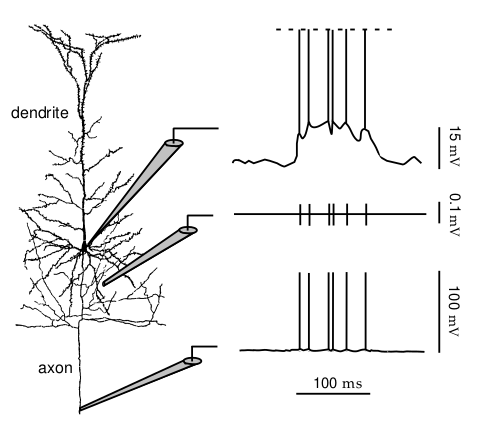
\includegraphics[height=65mm, width=75mm]{figure-18}
\end{figure}
\column{0.5\linewidth}
\begin{itemize}
\item $\sim$ 16 billion neurons in cortex
\item A neuron receives on the order of $10^{3}$ to $10^{4}$ synaptic inputs
\item Neurons communicate via action potentials in an all-or-nothing fashion
\item Post-synaptic potentials (PSPs) allow pre-synaptic action potentials to change post-synaptic membrane potential
\item PSPs can be positive or negative (excitatory or inhibitory)
\end{itemize}

\end{columns} 



\end{frame}


\begin{frame}{Integrate and fire (IF) neuron models}

\begin{figure}
\centering
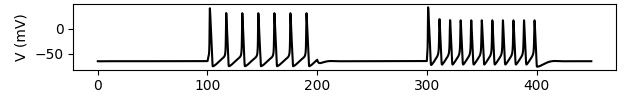
\includegraphics[width=140mm]{figure-19-1}
\end{figure}

\begin{figure}
\centering
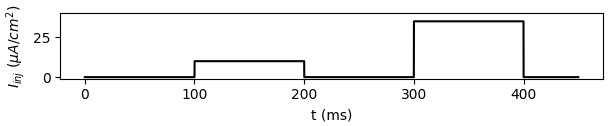
\includegraphics[width=140mm]{figure-19-2}
\end{figure}

Monte-Carlo simulations of neurons often use a Langevin equation:

\begin{equation*}
\tau\dot{V}(t) = g_{\ell}(E - V) + g_{\ell}\cdot \psi(V) + I(t)
\end{equation*}


\end{frame}

\begin{frame}{Monte-Carlo simulation of an integrate and fire model}

When $\psi(V) = g_{\ell}\Delta_{T}\exp\left(\frac{V-V_{L}}{\Delta_{T}}\right)$ we have the exponential integrate and fire model

\begin{figure}
\centering
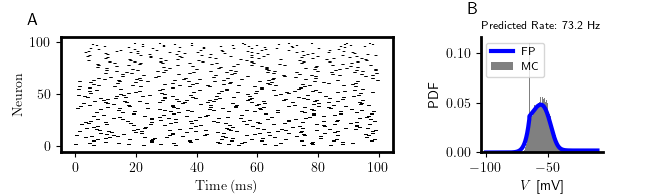
\includegraphics[width=140mm]{figure-3-1}
\end{figure}

Langevin equations have a corresponding Fokker-Planck equation 

\begin{equation*}
\frac{\partial P}{\partial t} = \frac{\sigma^{2}}{\tau}\frac{\partial^{2}P}{\partial V^{2}} + \frac{\partial}{\partial V}\left(\frac{V-E+\psi}{\tau}P\right)
\end{equation*}

which we can occasionally solve numerically

\end{frame}

\begin{frame}{Synaptic coupling can induce correlations in spiking activity}

\begin{columns}
\column{0.5\linewidth}
\begin{figure}
\caption{$N=1000$ densely coupled excitatory-inhibitory neurons}
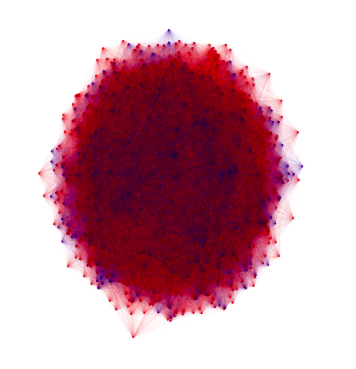
\includegraphics[height=60mm, width=70mm]{figure-17}
\end{figure}
\column{0.5\linewidth}
\begin{itemize}
\item When neurons are coupled $I(t) = F(t) + R(t)$
\item Non-trivial correlations then can arise from correlations in $F(t)$ and $R(t)$.
\item Dynamics of $I(t)$ depend strongly on the connectivity matrix $\mathcal{C}$
\item $\mathcal{C}$ itself is dynamic (synaptic plasticity)
\end{itemize}

\end{columns} 

\end{frame}


\begin{frame}{Synaptic coupling can induce correlations in spiking activity}

\begin{itemize}
\item For special $\mathcal{C}$, dynamical variables can remain uncorrelated between neurons
\end{itemize}


\begin{figure}
\centering
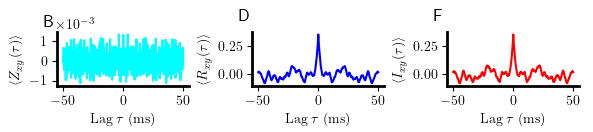
\includegraphics[width=140mm]{figure-12-1}
\end{figure}

\begin{itemize}
\item Uncorrelated neural activity captures irregular spiking seen \emph{in-vivo}
\item However correlated activity is thought to be fundamental to the neural code
\end{itemize}

\end{frame}

\begin{frame}{Linear response of the EIF model}

\begin{itemize}
\item Neurons are often modeled as heterogeneous Poisson processes
\item Heterogeneous Poisson processes have a time-dependent rate $r(t)$, which has a frequency response
\end{itemize}

\begin{figure}
\centering
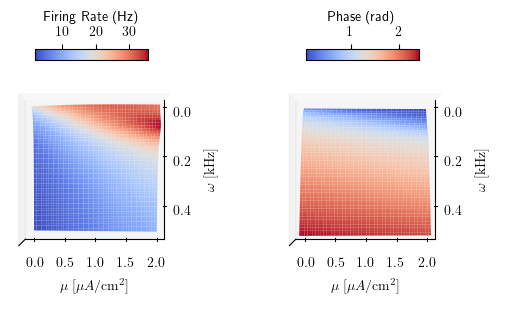
\includegraphics[width=100mm]{figure-4}
\end{figure}

\end{frame}

\begin{frame}{Predicting neuron correlations}
The linear response of $r(t)$ allows us to also estimate the matrix of cross-correlations $C_{kj}(\tau)$
from the synaptic connectivity $\mathcal{C}$
\begin{figure}
\centering
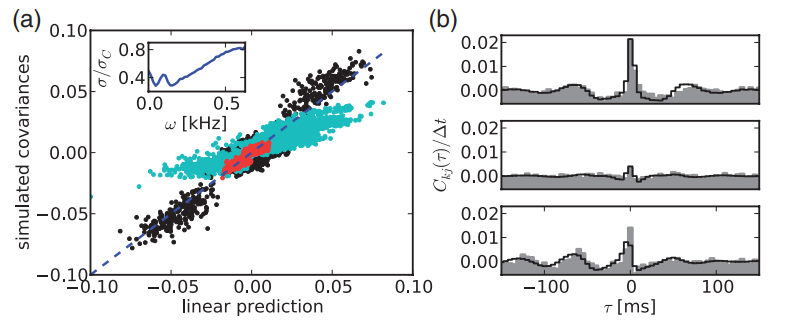
\includegraphics[width=110mm]{figure-20}
\end{figure}

This has important implications for brain-inspired machine learning

\end{frame}


\end{document}